\documentclass[12pt,a4paper]{report}

% Pacotes básicos
\usepackage{mathptmx}
\usepackage{indentfirst}
\usepackage[utf8]{inputenc}    % Permite acentuação
\usepackage[T1]{fontenc}       % Codificação correta das fontes
\usepackage[brazil]{babel}     % Idioma português
\usepackage{geometry}          % Configuração da página
\geometry{a4paper, top=2cm, bottom=2cm, left=2.5cm, right=2.5cm}
\usepackage{setspace}          % Espaçamento entre linhas
\usepackage{graphicx}          % Inserir imagens
\usepackage{hyperref}          % Links clicáveis
\usepackage{titlesec}          % Personalização dos títulos
\usepackage{array}             % Tabelas mais flexíveis
\usepackage{longtable}         % Tabelas longas
\usepackage{tikz}
\usetikzlibrary{positioning,shapes.geometric}

% Configurações do documento
\onehalfspacing               % Espaçamento 1.5
\hypersetup{
    colorlinks=true,
    linkcolor=blue,
    urlcolor=blue,
    pdftitle={Universidade Estadual do Norte Fluminense Darcy Ribeiro},
    pdfauthor={Davi Rodrigues Soares Machado},
}

\begin{document}
\begin{titlepage}
    \begin{center}
        
        
\includegraphics[scale=0.2]{imagens/uenf1.png}\\[1cm]
       
        {\large CENTRO DE CIÊNCIAS E TECNOLOGIAS}\\
        {\large LABORATÓRIO DE CIÊNCIAS MATEMÁTICAS}\\[4cm]

        {\large \textbf{Davi Rodrigues Soares Machado}}\\[4cm]

        {\large \textbf{Projeto da disciplina Paradigmas Orientados à Objetos para Desenvolvimento de Software: \\ Sistema de Agenda Escolar}}\\[4cm]

        Campos dos Goytacazes - RJ\\
        \today
    \end{center}
\end{titlepage}


% Sumário
\tableofcontents
\newpage


% Introdução -----------------------------------------------------------------------
\chapter{Introdução}
A proposta deste projeto consiste no desenvolvimento de um sistema de agenda escolar voltado para atender às demandas de uma rede de escolas. O objetivo central é oferecer uma ferramenta que permita a alunos, professores e outros profissionais da instituição visualizar e acompanhar informações essenciais, como distribuição de salas, organização de turmas, docentes responsáveis, além de outras funcionalidades que serão apresentadas com maior clareza na seção de \hyperref[sec:Diagrama]{Diagramas}.

Esse projeto servirá como simulação prática de desenvolvimento de um software,para a disciplina Paradigmas Orientados à Objetos para Desenvolvimento de Software (POODev), possibilitando a aplicação de conceitos aprendidos em disciplinas como Programação Orientada à Objetos, Banco de Dados e Análise e Projeto de Sistemas.Além disso, o desenvolvimento será registrado e versionado dentro da plataforma GitHub, no \href{https://github.com/DaviRodrish/Projeto-PooDev---Agenda-Escolar}{Repositório Github}, onde será possível acompanhar a evolução do sistema, de acordo com o \hyperref[sec:cronograma]{Cronograma}.


% Objetivos -------------------------------------------------------------------------
\chapter{Objetivos}
O projeto tem como objetivo central a organização da agenda escolar virtual de uma rede de escolas, integrando informações como alocação de salas,informações sobre disciplinas, professores e horários em uma única plataforma. O sistema também contará com recursos para os professores lançarem notas dos alunos, sendo possivel gerar um relatório onde cada aluno poderá acompanhar suas notas de cada bimestre. O sistema de notas poderá gerar boletins escolares bimestrais e anuais para um melhor acompanhamento das respectivas notas. 

\subsection*{Principais funcionalidades}
	\paragraph{Automatização da grade horária:}Com o objetivo de reduzir os possíveis erros humanos na alocação de salas e professores, o sistema ficará responsável pela melhor distribuição dentro de cada unidade escolar, auxiliado do coordenador de cada unidade escolar.
	\paragraph{Oferecer consultas personalizadas:} Cada usuário poderá acessar o sistema com o intuito de visualizar a agenda escolar baseada em filtros como: por aluno, professor, turma ou sala. Será possível acompanhar o cronograma escolar e acessar boletins de alunos, que serão gerados automaticamente após o professor responsável lançar as notas das disciplinas.
	\paragraph{Acesso disponível em multi plataformas:} O sistema poderá ser acessado por qualquer dispositivo com acesso a intert via navegador web ou mobile.


 
\section{Público Alvo}
O público-alvo do sistema é formado por todos os membros que participam do processo acadêmico e administrativo de uma escola, cada um com diferentes níveis de uso e necessidades específicas. Os coordenadores de curso serão um dos principais perfis responsáveis por montar e gerenciar a grade horária, alocar professores e organizar a distribuição de salas. Os professores, utilizarão o sistema para consultar suas disciplinas, horários e salas atribuídas, garantindo maior clareza na sua rotina de trabalho. Já os alunos terão acesso a própria agenda, com a possibilidade de acompanhar as disciplinas e horários de forma prática e acessível. Desse modo, o sistema visa atender de forma integrada os diferentes tipos de usuários,gerando uma maior organização e agilidade.


\section{Orçamento}
No orçamento abaixo foram levados em consideração o período de quatro meses de desenvolvimento do sistema, somado com o periodo de uso de um ano seguido.
\begin{figure}[!h]
	\centering
	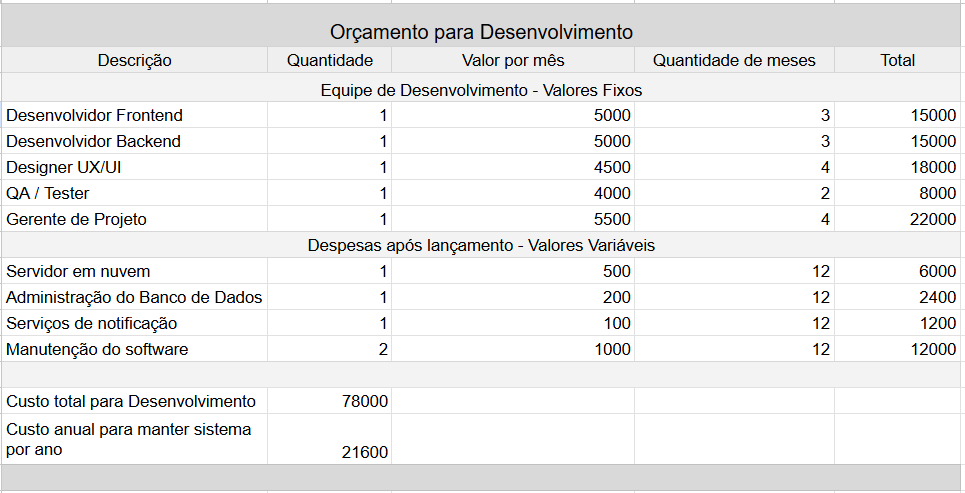
\includegraphics[width = \linewidth]{imagens/orcamento.png}
	\label{Orçamento}
	\caption{Orçamento}
\end{figure}



% Levantamento de Requisitos----------------------------------------------------------
\chapter{Levantamento de Requisitos}
Durante a primeira reunião, foram levantados alguns requisitos que foram listados abaixo, com a possibilidade do sistema de assinatura digital. 
\section{Requisitos Funcionais}
	\begin{itemize}
    \item RF01: Cadastrar professores, alunos, salas e disciplinas e unidades escolares.
    \item RF02: O login deve ser através de email e senha.
    \item RF03: O sistema deve atribuir diferentes níveis de permissão baseado no tipo de usuário
    \item RF04: Cada sala deve possuir informações de localização, capacidade e tipo
    \item RF05: O sistema deve alertar quando houver alguma incompatibilidade
    \item RF06: Cada usuário deve ter a capacidade de visualizar os relatórios referentes ao seu nível (ex. alunos - boletins e horario escolar; professores - turmas e horários)
    \item RF07: O sistema deve permitir exportar os relatórios em pdf
    \item RF08: Consultar grade horária por aluno, professor ou sala.
    \item RF09: Alocar salas a disciplinas em horários específicos.
    \item RF10: Impedir conflitos de agendamento.
    \item RF11: Gerir notas dos alunos, sendo possivel gerar relatorios com situaçao de aprovado ou reprovaado ou registro de notas.
    \item RF12: Sistema de assinatura digital dos professores e coordenadores.
	\end{itemize}

\section{Requisitos Não Funcionais}
	\begin{itemize}
    \item RNF01: O sistema deve ser responsivo e rápido.
    \item RNF02: O sistema deve apresentar telas intuitivas com navegação simples.
    \item RNF03: O sistema deve suportar pelo menos 200 usuários simultâneos.
    \item RNF04: O sistema deve criptografar senhas dos usuários.
    \item RNF05: O sistema deve implementar níveis de permissão de acordo com o perfil do usuário.
    \item RNF06: O sistema deve ser capaz de aumentar a capacidade de usuários e dados sem degradação significativa de desempenho.
    
	\end{itemize}

% Casos de Uso ----------------------------------------------------------------------

\chapter{Diagramas}
\label{sec:Diagrama}
\section{Diagrama de Caso de Uso}

Seguindo o diagrama abaixo, temos os principais casos de uso do sistema de agenda escolar. Começamos com as entidades: Aluno, Professor, Coordenador,Secretário e Pró Reitor, em que cada uma terá acesso a funcionalidades específicas dentro do sistema. Por exemplo, somente os professores poderão lançar e editar as notas dos alunos.

\begin{figure}[!h]
	\centering
	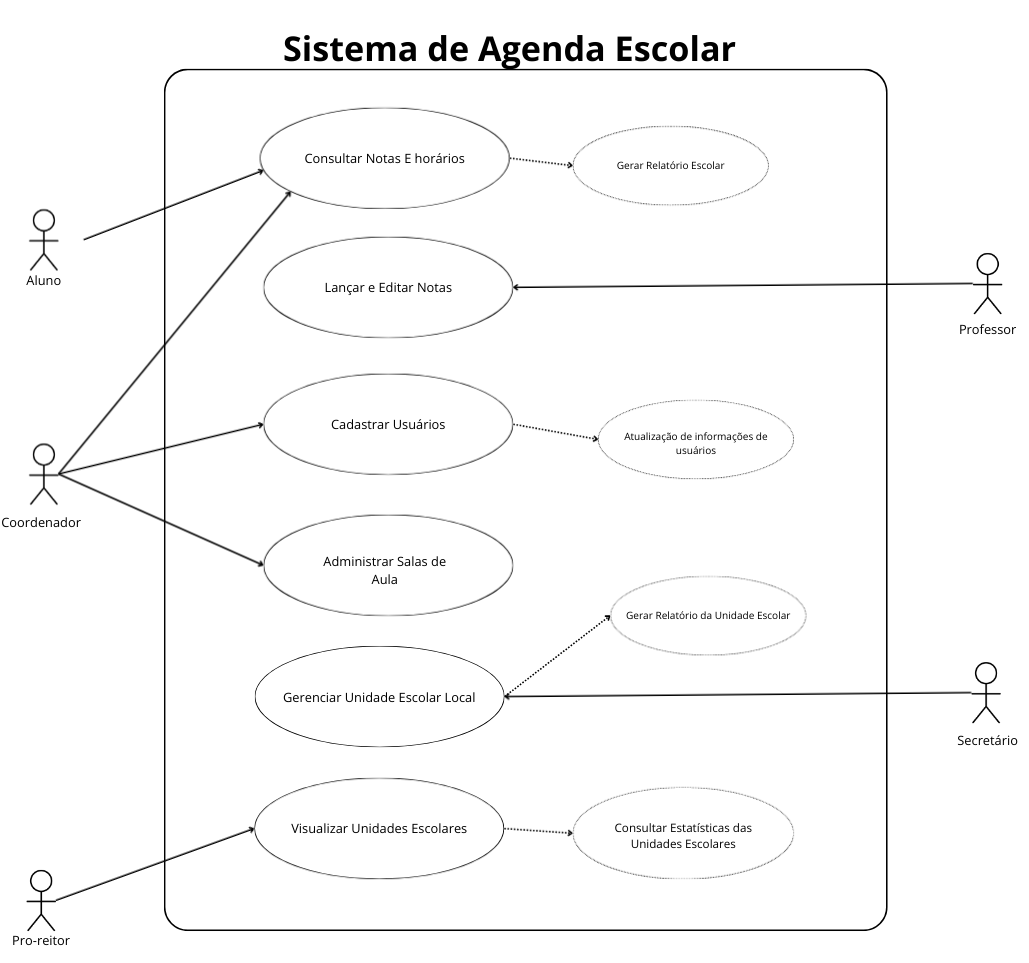
\includegraphics[scale=0.5]{imagens/casodeuso.png}
	\caption{Diagrama de Casos de Uso}
	\label{Diagrama de Casos de Uso}
\end{figure}

\section{Diagrama UML}
No diagrama UML, cada uma das classes é projetada com seus respectivos atributos e métodos.

\begin{figure}[!h]
	\centering
	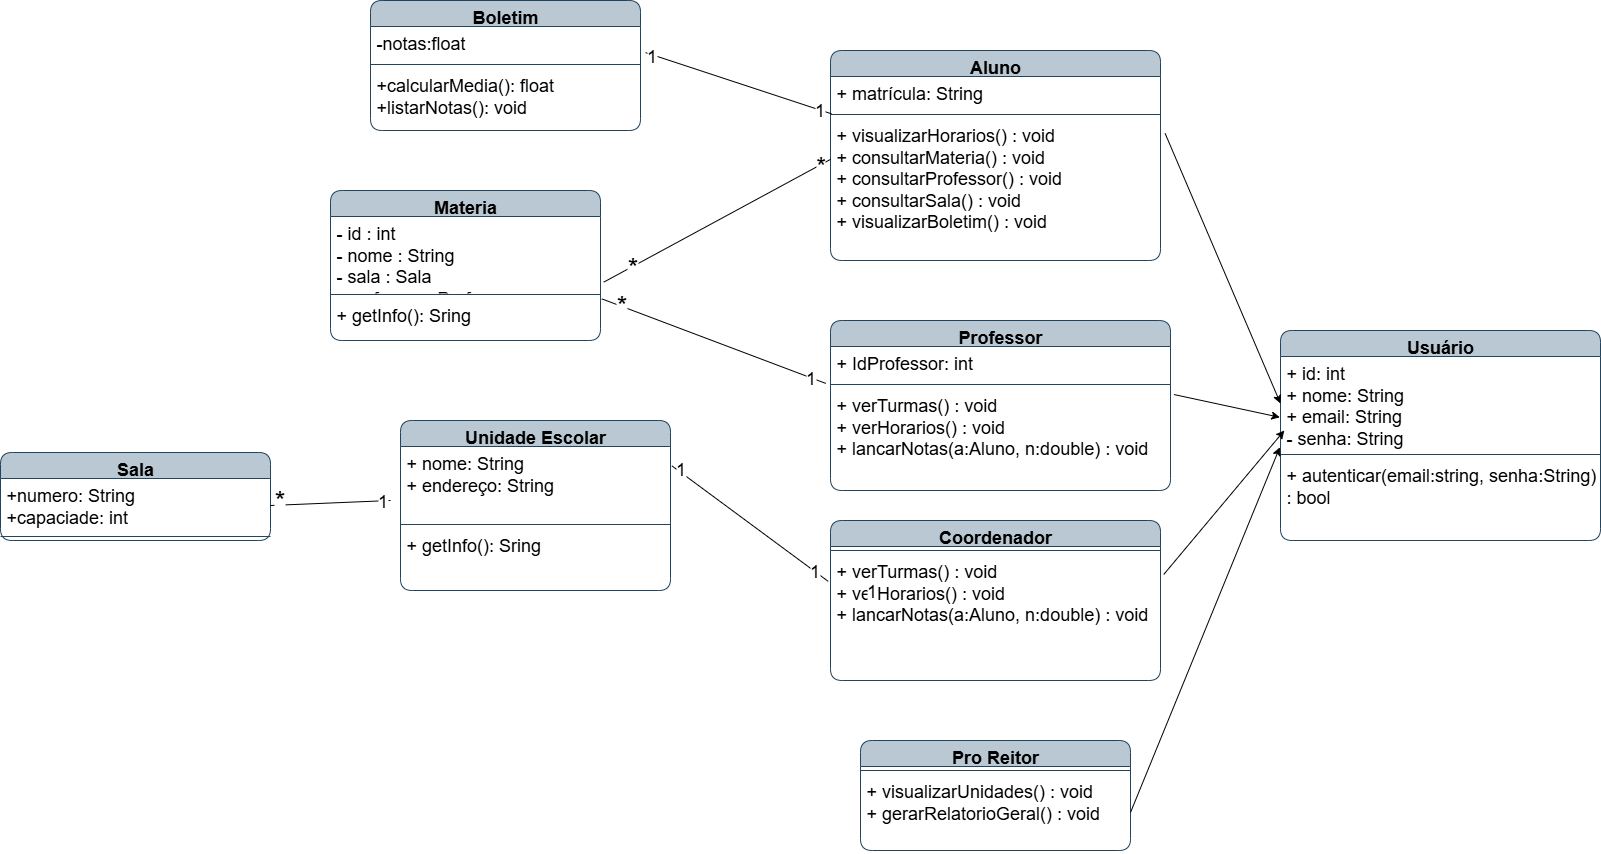
\includegraphics[width = \linewidth]{imagens/uml.png}
	\label{Diagrama UML}
	\caption{Diagrama UML}
\end{figure}
\newpage
\section{Diagrama Entidade Relacionamento}
\begin{figure}[h!]
\centering
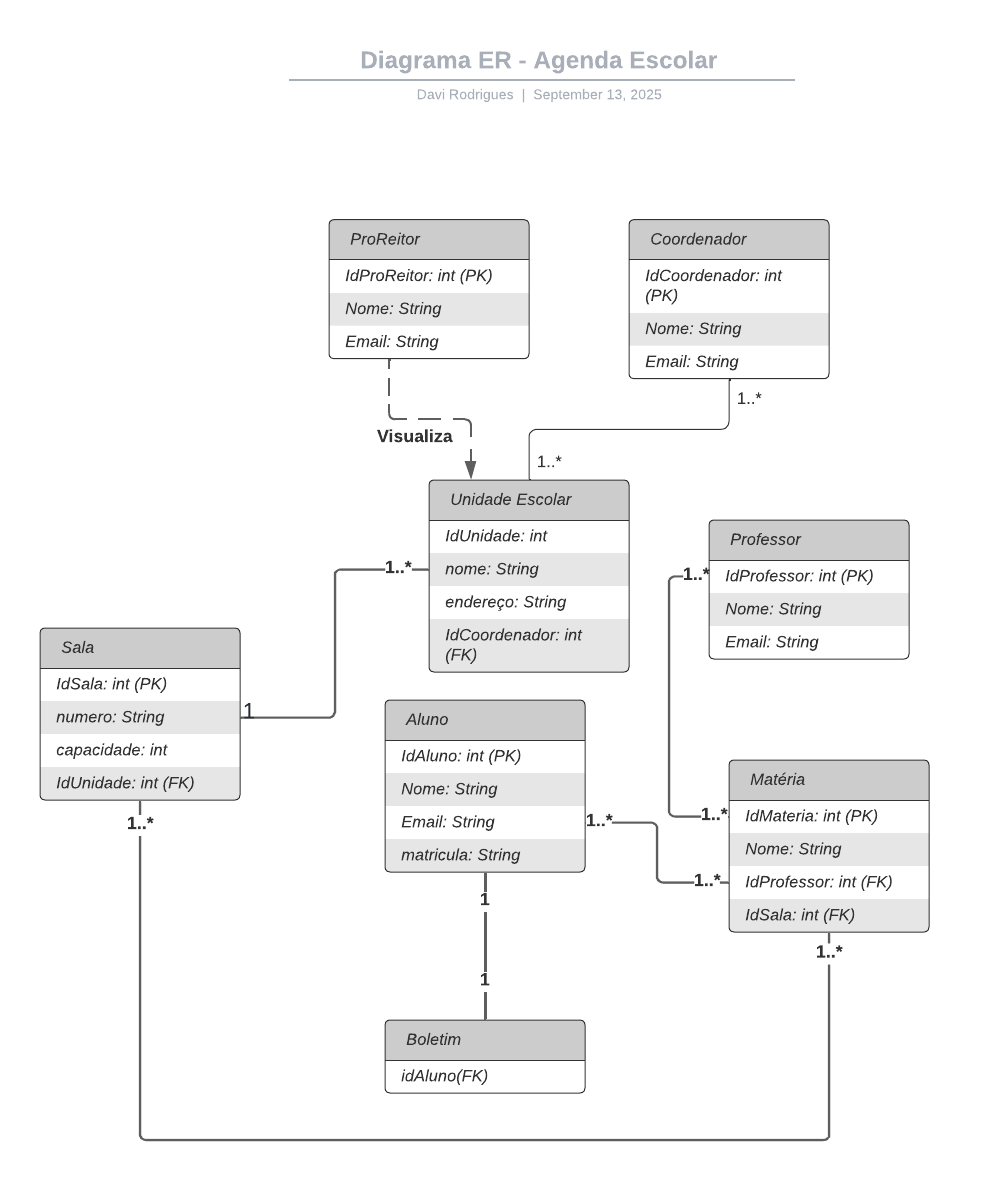
\includegraphics[width=\linewidth]{imagens/der.png}
\label{Diagrama Entidade-Relacionamento}
\caption{Diagrama Entidade-Relacionamento}
\end{figure}

% Arquitetura do Sistema -------------------------------------------------------------
\chapter{Arquitetura do Sistema}
\paragraph{Visão geral} O sistema foi projetado com base na arquitetura cliente-servidor, onde a aplicação é dividida em dois grandes blocos: a interface de apresentação (front-end) e a lógica de negócio (back-end). Esses blocos se comunicam através de uma API REST, permitindo maior flexibilidade, escalabilidade e manutenção.
O banco de dados relacional é utilizado para garantir a consistência das informações do sistema.

\paragraph{Fluxo de comunicação}
Basicamente, Quando um usuário estiver acessando o sistema, o front-end ficará responsável pelas interações com o usuário. Quando o usuário fizer uma solicitação, o front-end vai enviar requisições	ao back-end por meio de protocolos http. O back-end vai processar essas informações, consultando o banco de dados se necessário, e retorna ao front-end um arquiso JSON, que será visualizado pelo usuário como forma de resposta a solicitação.



% Tecnologias Utilizadas -------------------------------------------------------------
\chapter{Tecnologias Utilizadas}

\begin{itemize}
	\item \textbf{Back-end:} A linguagem escolhida para o desenvolvimento foi a linguagem Python.
	\item \textbf{Front-end:} O front-end servirá como ferramenta de visualização para o sistema e será desenvolvido principalmente com React e Tailwind CSS.
	\item \textbf{Banco de Dados:} PostgreSQL local
	\item \textbf{Controle de Versão:} Todo o processo será documentado e versionado dentro da plataforma github, que poderá ser acessada através do \href{https://github.com/DaviRodrish/Projeto-PooDev---Agenda-Escolar}{Repositório Github}
\end{itemize}

% Calendário -------------------------------------------------------------------------
\chapter{Cronograma}
\label{sec:cronograma}

Para melhor entendimento, o cronograma de desenvolvimento foi dividido em dois bimestres, sendo o primeiro focado em backend e integração com banco de dados, e o segundo focado no frontend e nos testes de aplicação. Em ambas etapas, no final de cada semana do mês, uma reunião com cliente irá acontecer, onde será mostrado cada nova parte incluída no sistema.  

\vspace{2cm}

\begin{figure}[!h]
\centering
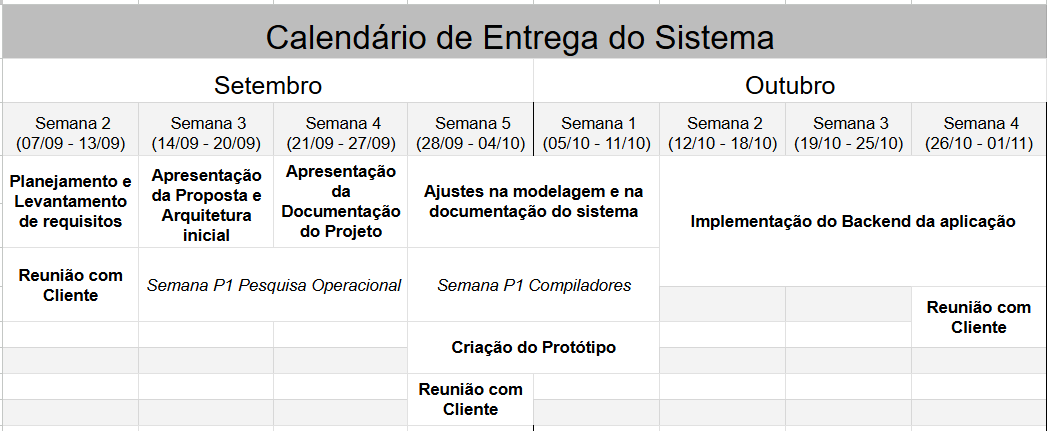
\includegraphics[width = \linewidth]{imagens/Calendario1bi.png}
\caption{Cronograma do Primeiro Bimestre de Desenvolvimento}
\label{Cronograma do Primeiro Bimestre de Desenvolvimento}
\end{figure}

\begin{figure}[!h]
\centering
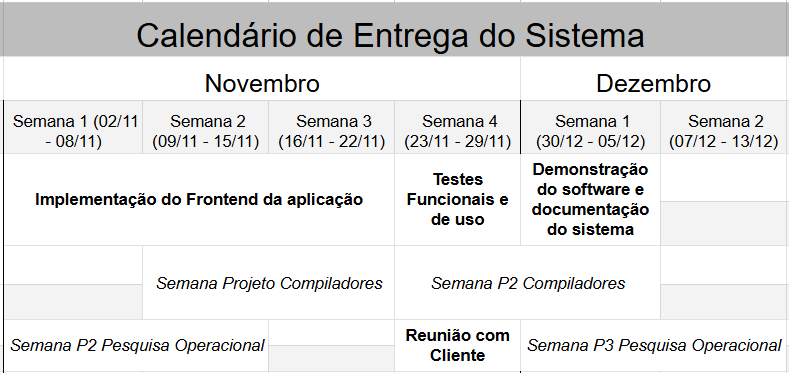
\includegraphics[width = \linewidth]{imagens/Calendario2bi.png}
\caption{Cronograma do Segundo Bimestre de Desenvolvimento}
\label{Cronograma do Segundo Bimestre de Desenvolvimento}
\end{figure}


\end{document}
